\chapter{Data and Models}
\label{chap:datamodels}

\section{Data}

The proposed research will address the question of machine learning integration by experimenting with documentary and descriptive data. Using field data will 1) reveal how current annotation methods affect the performance of NLP systems, 2) test the practicality of incorporating machine learning into the documentary and descriptive workflow, 3) demonstrate that IGT output of documentary and descriptive projects is sufficient to train machine learning models, and 4) enrich the selected data with the results of the experiments.
%A consensus among LDD practitioners is that more documented data is always better to support linguistic description or revitalization. This holds true for NLP as well: the more training data, the better the results. Yet, the combination of funding limitations and lack of integrated machine learning assistance means that the amount of interlinearized data that LDD projects is almost always less than what is collected and transcribed. 

The selected data corpora are representative of a range of typical documentary and descriptive projects. They consist of manually interlinearized glossed texts (IGT) from the seven under-documented and endangered languages presented in Table \ref{tab:langs}.   

\bgroup
\def\arraystretch{1.25}
\begin{table}[h!]
    \begin{center}
    \begin{tabular}{lcccccc} 
    \textbf{Language} & \textbf{ISO} & \textbf{Family} & \textbf{Morphology} & \textbf{Status} \\
    \hline
    Alas & btz & Austronesian & Agglutinative & Stable \\
    %\hline
    Arapaho & arp & Algonquian & Polysynthetic & Severely Endangered  \\
    %\hline
    Lamkang & lmk & Sino-Tibetan & Agglutinative & Endangered/Stable   \\
    %\hline
    Lezgi & lez & Nakh-Daghestanian & Agglutinative & Vulnerable \\
    %\hline
    Manipuri & mni & Sino-Tibetan & Agglutinative & Vulnerable  \\
    %\hline
    Natügu & ntu & Austronesian & Isolating & Stable \\
    %\hline
    Tsez & ddo & Nakh-Daghestanian & Agglutinative & Endangered   \\
    
	\end{tabular}
	\caption[Data]{Language name, ISO 639-3 code, language family, predominant morphological type, endangerment status.}
	\label{tab:langs}
\end{center}
\end{table}


\subsection{Languages} 

The selected languages are spoken across five continents.
%, with populations of speakers ranging from a few hundred to about two million. 
Published linguistic resources are limited, meaning all these languages are under-documented. Information about speaker population and endangerment status was retrieved from the \emph{Ethnologue} \citep{eberhard_ethnologue:2020} and \emph{Catalogue of Endangered Languages} \citep{elcat_2020}.
%UNESCO’s \underline{Atlas of Endangered Languages} \citep{moseley_atlas_2010}.

\paragraph{Alas.}
Alas [btz] (Alas-Kluet, Batak Alas, Batak Alas-Kluet) belongs to the Malayo-Polynesian branch of the Austronesia family. It is spoken by 200,000 people on the Indonesian island of Sumatra. It is unclear if the three dialects (Alas, Kluet, and Singkil) constitute one language. The selected corpus is from the Alas dialect. It features reduplication, infixation, and some circumfixation. The corpus consists of 12 transcribed texts and one set of elicited sentences written with the Indonesian orthography.

\paragraph{Arapaho.}
Arapaho [arp] is an Algonquian language spoken by about 1,000 people in Wyoming and Oklahoma, USA, but spoken fluently by less than 200. It is a highly polysynthetic, with as much information as possible going into the verb's morphology \citep{cowell_arapaho_2008}. This includes noun incorporation where special forms of certain nouns become part of the verb. The corpus contains texts and elicited sentences documented from the 1880s until the present day, including a few translated texts. They are written in the Arapaho orthography. Most of the data is available through the Endangered Languages Archive.\footnote{https://elar.soas.ac.uk/Collection/MPI189644}

\paragraph{Lamkang.} 
Lamkang [lmk] is a Northern Kuki-Chin Tibeto-Burman language. Depending on the primary source of population numbers, speakers are estimated between 4 to 10 thousand people. Speakers live primarily in Manipur, India but also in Burma \cite{lamkang_2007}. Its endangerment status is also not clear. It tends toward agglutination with many stem-stem patterns to signal syntactic categories. Many morphemes are written as seperate words in the corpus. There is limited literacy material available. The corpus is accesible through the Computational Resources for South Asian Languages (CoRSAL) digital archive at the University of North Texas.\footnote{https://digital.library.unt.edu/explore/collections/SAALT/}

\paragraph{Lezgi.} 
Lezgi [lez] (Lezgian) belongs to the Lezgic branch of the Nakh-Daghestanian (Northeast Caucasian) family. It is spoken by over 400,000 speakers in Russia and Azerbaijan. Lezgi is an highly agglutinative language with overwhelmingly suffixing morphology. The corpus contains oral texts in the endangered Qusar dialect of Azerbaijan. This dialect differs from the standard written dialect in a few ways, such as a locative case suffix borrowed from Azerbaijani which is used alongside the native inessive case suffix with the same meaning. The texts are transcribed into the language's Cyrillic orthography. The corpus is being deposited at SIL Language and Culture Archives.

\paragraph{Manipuri.}
Manipuri [mni] (Meitei, Meetei) belongs to the Tibeto-Burman branch of the Sino-Tibetan family. It is spoken by nearly two million people, primarily in the state of Manipur, and is one of India's official languages. It has nevertheless been classified as vulnerable to extinction by UNESCO. It is a tonal language and has weakly suffixing, agglutinative morphology \citep{Chelliah-1997}. It is the only Tibeto-Burman language in India with its own script, but the corpus was transcribed with the international Phonetic Alphabet (IPA). The corpus is available through the Computational Resources for South Asian Languages (CoRSAL) digital archive.\footnote{https://digital.library.unt.edu/explore/collections/MDR/}

\paragraph{Natügu.}
Natügu [ntu] belongs to the Reefs-Santa Cruz group in the Austronesian family. It is spoken by about 4,000 people in the Temotu Province of the Solomon Islands. It has a mainly agglutinative morphology with complex verb structures \citep{naess_ntu_2008}. The corpus contains transcribed narratives and a large written text. The data is available through SIL Language & Culture Archives\footnote{https://www.sil.org/resources/search/language/ntu} or is being deposited at the Pacific and Regional Archive for Digital Sources in Endangered Cultures (PARADISEC).

\paragraph{Tsez.}
Tsez [ddo] (Dido) belongs the Tsez-Hinukh branch of the Nakh-Daghestanian family. It is spoken by about 12,500 speakers in Daghestan, Russia. It has a rich agglutinative, suffixing morphology. The corpus is made up of folklore. It is part of the Tsez Annotated Corpus Project \citep{abdulaev-tsezcorpus-2010}. It is available online\footnote{https://tsezacp.clld.org/} and is stored and preserved by Zenodo.\footnote{zenodo.org}

\subsection{Corpora}

The data was selected primarily to represent a range of “typical” outputs by documentary and descriptive projects. Less effort was made to represent typological structures, geographic areas, or a range of language families. No effort was made to include a range of genre and origin; the texts are mostly narratives that were transcribed from recorded speech. Because the sample of languages is small, the proposed research will avoid sweeping claims that may depend on linguistic typology or discourse genre. 
The corpora were generously shared in the form of backup XML or CSV files. The rights holders gave informed consent to use the data for the proposed research. 
%The data providers also agreed to be available to answer questions about their projects and conduct error analysis when necessary.

In most cases, more data was recorded and transcribed than could be interlinearized within the project's budget. Only the Arapaho and Tsez corpora can be considered completed (though missing annotations were found in both during preprocessing). Each project's unique priorities and workflow resulted in different proportions of data that were fully segmented and glossed, as shown in Table \ref{tab:goldstandard}.

\begin{table}[hb]
    \centering
    \begin{tabular}{l|r|rc}
         \textbf{Language} & \textbf{Tokens} & \multicolumn{2}{c}{\textbf{Gold}} \\
         \hline
         Alas & 4.5K & 3,775 & 85\%  \\
         % 4462 btz actual number of tokens 
         % segmented and glossed: 3775/4462 = 0.846
         % translated: 302/303
         \hline
         Arapaho & 300K & 202,993 & 70\% \\
         % 294,774 arp actual number of tokens
         % segmented and glossed: 202993/294774 = 0.688
         \hline
         Lamkang & 101K & 50,252 & 50\% \\
         % segmented & glossed: 50252/101005 = 0.497
         % translated: 8629/8640 = 0.998
         \hline
         Lezgi & 14K & 13,353  &  94\% \\
        % 14175 lez actual number of tokens
        % segmented & glossed: 13353/14175 = 0.942
        % translated: 1531/1532
         \hline
         Manipuri & 12K & 11,907 & 98\% \\
        % 12139 mni actual number of tokens 
        % segmented & glossed: 11907/12139 = 0.980
        % translated: 1784/1785
         \hline
         Natügu & 16.5K & 13,925 &  84\%  \\
        % 16520 ntu actual number of tokens 
        % segmented & glossed: 13925/16520 = 0.842
        % translated: 1541/1542
         \hline
         Tsez & 53K & 53,145 & 100\%  \\
        % 53145 ddo actual number of tokens 
        % segmented & glossed: 53145/53145 = 1.0
        % translated: 
    \end{tabular}
    \caption[Corpora Sizes]{Corpora Sizes. The approximate token count does not include punctuation, digits, or proper names (when tagged as such) which are often left unannotated but can be easily supplied. The gold standard data are tokens that were fully segmented and glossed, shown as a number and as a percentage of corpus.}
    \label{tab:goldstandard}
\end{table}

%\begin{table}
%    \centering
%    \begin{tabular}{lccc}
%        \textbf{Language} & \textbf{Seg/Gloss} & \textbf{Translated} & \textbf{Ratio}\\
%        \hline
%        Alas & 75\% & 100\% & 3:4 \\
%        \hline
%        Arapaho &  &  \\
%        \hline
%        Lezgi &  &  \\
%        \hline
%        Manipuri &  &  \\
%        \hline
%        Natügu &  &  \\
%        \hline
%        Tsez & 100\% & 100\% & 1:1 \\
%    \end{tabular}
%    \caption[Proportions of Completed Interlinear Lines]{The percentage of lines in each corpus that were completely segmented and glossed (Seg/Gloss) and the percentage that was translated.}
%    \label{tab:proportion}
%\end{table}

Each corpus required preprocessing because of errors, typos, changing analyses, or variable formatting. Even projects that employed the same software tool had variable formatting. For example, both Natugu and Bahasa Alas have circumfixing, but in one corpus the prefixed part was labeled as a circumfix and the suffixed part as a suffix, while the other corpus took the opposite approach. 
%Other issues arose from the variety of fonts for models that only accept ASCII characters. 

Gold standard data for training and testing was produced by filtering incomplete annotations. Only tokens that were completely segmented and glossed, and only sentences that were translated are included in the gold standard for the relevant experiments. The resulting data sizes are given in Table \ref{tab:goldstandard}.

The projects that produced the corpora spent different amounts of time on interlinearization, had different short-term goals, and varied by team size, team members' education or linguistic training. For example, the Alas corpus was produced in a matter of months while the Arapaho and Natügu corpora were produced by projects that have extended over many years. These two corpora, as well as the Tsez corpus, were annotated by teams with multiple linguists and native speakers. In contrast, the projects that produced the Alas corpus and most of the Lezgi corpus had one linguist and one or two native speaker annotators. The smaller, shorter projects were usually not able to provide as much training to annotators. Most projects were undertaken with the primary goal of documenting and describing the language, but the shorter-term goal of the Alas project is to support literacy efforts while most of the work on the Lezgi corpus was done to support an MA thesis on verbs. These factors are reflected in the quality of the interlinearization. For example, in the Lezgi corpus only verbs were consistently annotated by a trained linguist. The rest was annotated by a native speaker with minimal linguistic training and, therefore, contains more errors and inconsistencies. 

The proposed research is centered around issues that arise from the quality of interlinearization. 
%Variation can be problematic. One kind of variation is the typological differences among the languages. Another kind of variation arises in the IGT corpora. They vary in size and quality. The issues due to size are self-evident and the consensual answer is that more data is better. Issues of quality will be brought to focus in the proposed research. These issues are varied. 
The research assumes certain issues are more significant than others. The less significant ones, such as typos in glosses and inconsistent morpheme segmentation, are ignored or handled during preprocessing. The more significant issues are different segmentation strategies (surface vs. canonical) and different proportions of completed lines of interlinearization.


\section{Models}
\label{sec:models}

The proposed research will use three supervised machine learning systems. All three have achieved state-of-the-art NLP results in low-resource settings. They include two feature-based (CRF, SVM) and one neural system (Transformer). 
%The models will be trained for three tasks: 1) morpheme segmentation and glossing, 2) translation, and 3) inflectional paradigm induction.

\paragraph{Conditional Random Fields (CRF).} The best performing non-neural model for sequence prediction such as morpheme segmentation and glossing is Conditional Random Fields (CRF) \citep{lafferty_conditional_2001,muller_efficient_2013,ruokolainen_comparative_2016}. A linear-chain CRF \citep{lafferty_conditional_2001} will be implemented with \textit{CRFsuite} \citep{okazaki2007} and its Python API.\footnote{\url{https://python-crfsuite.readthedocs.io/en/latest/}} 
The CRF is a sequence classifier that considers the whole sequence of symbols (words, letters, glosses, etc.) when making an individual prediction. It tries to optimize the probability of a complete sequence of labels, where each individual label is given a conditional probability based on the previous label and an arbitrary number of surrounding inputs. %\mans{This is tricky to word correctly. A CRF tries to optimize the probability of a complete sequence labeling, where each individual label gets a conditional probability based on the previous label and arbitrary surrounding inputs. Let's make sure to revisit this at some point.} 
The CRF has performed well on boundary detection (segmentation) and labeling (glossing). 

%CRF learn to predict sequences with the help of pre-chosen features extracted from the data. Logistic regression allows the predictions to be generalized from arbitrary and possibly dependent features \citep{ruokolainen_supervised_2013}.  
%According to Ruokolainen et al. \cite{ruokolainen_comparative_2016}, discriminative models, compared to generative models, generalize better and optimize boundary detection.
%The strength of a discriminative model such as the CRF lies in its ability to examine more features than the ones extracted for the current symbol. 
%It assigns arbitrary weights to the features during training. 

\begin{figure}
    \centering
    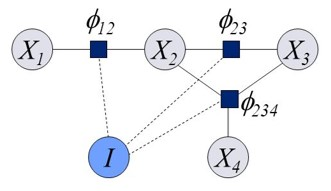
\includegraphics[width=6cm]{figs/CRF.jpg}
    \caption[Conditional Random Fields]{Conditional Random Fields sequence classifier.\footnote{source: www.slideplayer.com/slide/9361527}}
    \label{fig:CRF}
\end{figure}

For the CRF (Fig. \ref{fig:CRF}), predictions are scored over the whole sequence and then transformed into a probability distribution. The conditional distribution of the output sequence {\bf y}, given the input {\bf x} can be modeled as

\begin{equation}
p(\vect{y}|\vect{x}) = \frac{1}{Z} \textrm{exp}\Big(\sum_{i=1}^n\phi(y_{i-1}, y_i,\vect{x},i)\Big)
\end{equation}

\noindent where $\phi$ is the feature extraction function which can be expressed through a sum of $k$ individual component functions

\begin{equation}
\phi(y_{i-1}, y_i,\vect{x},i) = \sum_k w_k f_k(y_{i-1}, y_i,\vect{x},i)
\end{equation}

\noindent Here, $Z$ is the ``partition function'' which normalizes the expression to a proper distribution over all possible taggings given an input. 

\paragraph{Support Vector Machine (SVM).} The proposed research will experiment with a pipeline method that first segments morphemes with the CRF and then glosses them with a Support Vector Machine (SVM) \citep{svm_cortes}. The SVM will label only after segmentationg is done by the CRF, using its own feature scheme. The SVM will be implemented as a multi-class linear SVM using the LIBLINEAR package \citep{fan2008}. It creates hyperplanes to separate the data into classes. The optimal hyperplane is found by maximizing the margin between the closest data points in each class, as illustrated in Figure \ref{fig:SVM}. These data points are the support vectors. Like CRF, the SVM learns from extracted features.

%\Mans{You should make clear that we used an SVM as a labeler after the segmentation was done, using some feature scheme. Otherwise a reader will be confused as to how you an SVM as a sequence labeler (possible, but not normally done) vs. a CRF which is inherently a sequence labeler.}

\begin{figure}
    \centering
    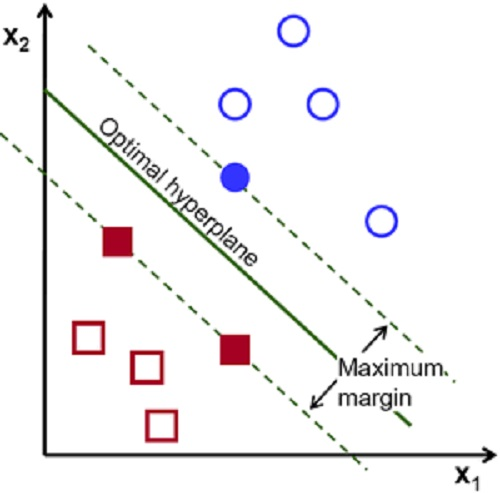
\includegraphics[width=5cm]{figs/SVM1.jpg}
    \caption[Support Vector Machine]{A Support Vector Machine (SVM).\footnote{source: www.aitrends.com/ai-insider/support-vector-machines-svm-ai-self-driving-cars/}}
    \label{fig:SVM}
\end{figure}

\paragraph{Transformer.} The proposed research will use the neural transformer model \citep{vaswani_attention_2017} in all three studies. Transformers have achieved promising results for NLP in low-resource languages \citep{abbott_towards_2018,Martinus2019AFO}. 
%Like most neural models, the transformer’s main drawback in low-resource settings is its sensitivity to hyper-parameters.
The proposed research will use the parameters of the fairseq \citep{ott2019fairseq} implementation that have been successful for NLP in low-resource settings \citep{wu2020applying}.

%The standard Transformer encoder consists of identical layers, each of which has a multi-headed self-attention layer, and  one feed-forward layer. A residual connection is around two sub-layers, followed by layer normalization.

The Transformer is a encoder-decoder model that uses Attention to boost speed and performance, as illustrated in Figure \ref{fig:transformer}. Attention allows the model to look at different elements in the sequence to help it encode/decode a given element before feeding it to the next encoder. The decoder has an additional attention layer that allows it to focus not only on the input sentence but also on the ouput sequence up to the element it is decoding. The order of elements in the sequence is represented as an embedding which is input to the encoder/decoder. 

\begin{figure}
    \centering
    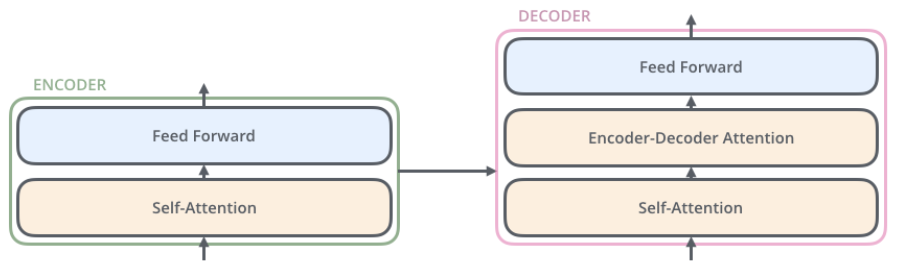
\includegraphics[width=14cm]{figs/Transformer_simplified.png}
    \caption[Transformer]{The Transformer encoder.\footnote{source: http://jalammar.github.io/illustrated-transformer/}}
    \label{fig:transformer}
\end{figure}

\paragraph{LSTM encoder-decoder.} In one study the proposed research will use a LSTM sequence-to-sequence model with exact hard monotonic attention for character-level transduction \citep{wu-cotterell-2019-exact}. This model is used as neural comparison to the Transformer. 

%DESCRIBE (used for IGT2P).